%% Beginning of file 'RubinAsteroids.tex'
%%
%%
\documentclass[linenumbers,trackchanges,twocolumn]{aastex701}
%%
\newcommand{\vdag}{(v)^\dagger}
\newcommand\aastex{AAS\TeX}
\newcommand\latex{La\TeX}


\usepackage{amsmath}
\usepackage{rotating}
\graphicspath{{./}{../}}
\usepackage{listings}
\usepackage{xcolor}
\usepackage{subcaption}
\usepackage{placeins} % For \FloatBarrier

\lstdefinelanguage{SQL}{
  keywords={SELECT, FROM, WHERE, AND, OR, INSERT, INTO, VALUES, UPDATE, SET, DELETE, JOIN, ON, CREATE, TABLE, AS, DISTINCT, GROUP, BY, ORDER, DESC, ASC, INNER, LEFT, RIGHT, OUTER, LIMIT},
  sensitive=false,
  comment=[l]{--},
  morecomment=[s]{/*}{*/},
  morestring=[b]',
  morestring=[b]"
}

\lstset{
  language=SQL,
  basicstyle=\ttfamily\small,
  keywordstyle=\color{blue}\bfseries,
  commentstyle=\color{gray},
  stringstyle=\color{orange},
  showstringspaces=false,
  breaklines=true
}

\begin{document}

\title{Prioritising Follow up of Potentially Hazardous Asteroids using Bayesian Methods}




\author[0009-0004-0059-3229]{Devanshi Singh}
\affiliation{DiRAC Institute and the Department of Astronomy, University of Washington, 3910 15th Ave NE, Seattle, WA, 98195, U.S.A.}
\email{ds2004@uw.edu}

\author[orcid=0000-0001-5250-2633]{\v{Z}eljko Ivezi\'{c}}
\affiliation{DiRAC Institute and the Department of Astronomy, University of Washington, 3910 15th Ave NE, Seattle, WA, 98195, U.S.A.}
\email{ivezic@astro.washington.edu}

\author[orcid=0000-0003-1996-9252]{Mario Juri\'{c}}
\affiliation{DiRAC Institute and the Department of Astronomy, University of Washington, 3910 15th Ave NE, Seattle, WA, 98195, U.S.A.}
\email{mjuric@astro.washington.edu}




%\input{auth}


\begin{abstract}
We describe the whatever-tf-we're-calling-this-package a 

\end{abstract}


\keywords{\uat{Small Solar System bodies}{1469} --- \uat{Main belt asteroids}{2036} -- \uat{Asteroid rotation}{2211} --- \uat{Lightcurves}{918} --- \uat{Two-color diagrams}{1724} --- \uat{Photometry}{1234} --- \uat{Optical astronomy}{1776}}


\section{Introduction}
\label{sec:intro}

The discovery of Near-Earth Objects (NEOs), small solar system bodies with perihelia less than \( 1.3 \, \text{au} \), has accelerated dramatically over the past two decades, driven by Congressional mandates to survey \( 90\% \) of NEOs larger than \( 140 \, \text{metres} \) (the George E. Brown, Jr. NEO Survey Act, 2005). The Minor Planet Center (MPC) coordinates this effort globally through the Near-Earth Object Confirmation Page (NEOCP), a continuously updated list of newly discovered candidates requiring prioritised follow-up observations to confirm or rule out their NEO status. The primary tool currently used to score and classify these candidates is the digest2 code (Keys et al. 2019), which assigns a pseudo-probability score (\( D2 \)), between \( 0 \) and \( 100 \) based on the consistency of a short-arc tracklet with known orbital populations.

While digest2 has served the community reliably for over a decade, it was designed and calibrated for a survey landscape and magnitude depth limit that is about to change dramatically. The Rubin Observatory’s Legacy Survey of Space and Time (LSST) is expected to increase the nightly submission rate to the NEOCP by a factor of roughly eight compared to present day, contributing approximately \( 129 \) new candidates per night in its first year alone (Wagg et al. 2024). Of these, only around \( 8.3\% \) will be genuine NEOs, with the dominant contaminant being a background of previously undiscovered, faint Main Belt Asteroids (MBAs). This represents a fundamental challenge that the digest2 was designed to handle hundreds of candidates, not thousands, and its underlying population model, the Pan-STARRS Synthetic Solar System Model (S3M; Grav et al. 2011), is known to overestimate the number of solar system objects by approximately \( 25\% \) compared to current observations. As Wagg et al. (2024) demonstrated, even requiring a digest2 score of \( 90 \) or above only raises the NEO purity to \( 8.1\% \), making it ineffective as a standalone filter in the Rubin era.

What is needed is a new classification framework: one that uses the observed sky-plane properties of a tracklet, particularly its rates of motion in ecliptic coordinates together with a proper probabilistic model of the different asteroid populations, to produce a more robust and interpretable NEO score. In this work, we develop such a framework using a Bayesian nearest-neighbour density estimation approach applied to the four major dynamical populations of small solar system bodies: Near-Earth Objects (NEOs), Main Belt Asteroids (MBAs), Jupiter Trojans, and Trans-Neptunian Objects (TNOs). We construct probability maps over a fine grid in ecliptic rate-of-motion space, and use these maps to assign a population membership probability to any observed tracklet. We validate our approach against simulated data from S3M and test our classifier's performance against that of digest2 using real NEOCP candidates and Rubin discoveries.





\section{Methods}

\label{sec:methods}

include plot of all asteroids, with mars cross struck, also some sections in results about how neos and mars crossers are NOT very easy to distinguish. 

include section why am i not using neomod3, show comparison plot of NEOs between them to show slight difference.

orbital element comparison plot from pre cloned s3m and new cloned s3m

ooh and a version of zeljkos plot but overlaying the lines for all the diff. categories -- fig 14. from ivezic 2001.

so the 4 panel d ddot plots for mj, re do them but for cloned orbital elements maybe?? with the probability score on the side? is it even possible???

also include s3m population red berry candy looking plot


\subsection{Solar System Model and Population Selection}
\label{sec:popmodel}

Our starting point is the Pan-STARRS Synthetic Solar System Model (S3M; Grav et al. 2011), which serves as the baseline model of the Solar System used throughout this work. S3M contains about 14 million simulated Keplerian orbits spanning the major dynamical populations of small bodies. For each of the four populations of interest, NEOs, MBAs, Jupiter Trojans, and TNOs, we construct dataframes from S3M using four orbital parameters as our primary axes: absolute magnitude H, semi-major axis a, eccentricity e, and inclination i.

From these we build four-dimensional binned arrays that encode the population distributions for subsequent use in the density estimation step.
As a validation step, we first reproduce key figures from Ivezić et al. (2001), specifically the distribution of asteroid positions in ecliptic coordinates as observed by the Sloan Digital Sky Survey. This serves as a unit test of our orbital propagation and population selection pipeline before we proceed to more complex analyses.

Figure~\ref{fig:helio_map} shows the heliocentric ecliptic-plane distribution of all four populations at the Spring Equinox epoch (2025 March 21), providing an intuitive overview of the spatial scales and orbital architectures involved.

\begin{figure*}[ht!]
\centering
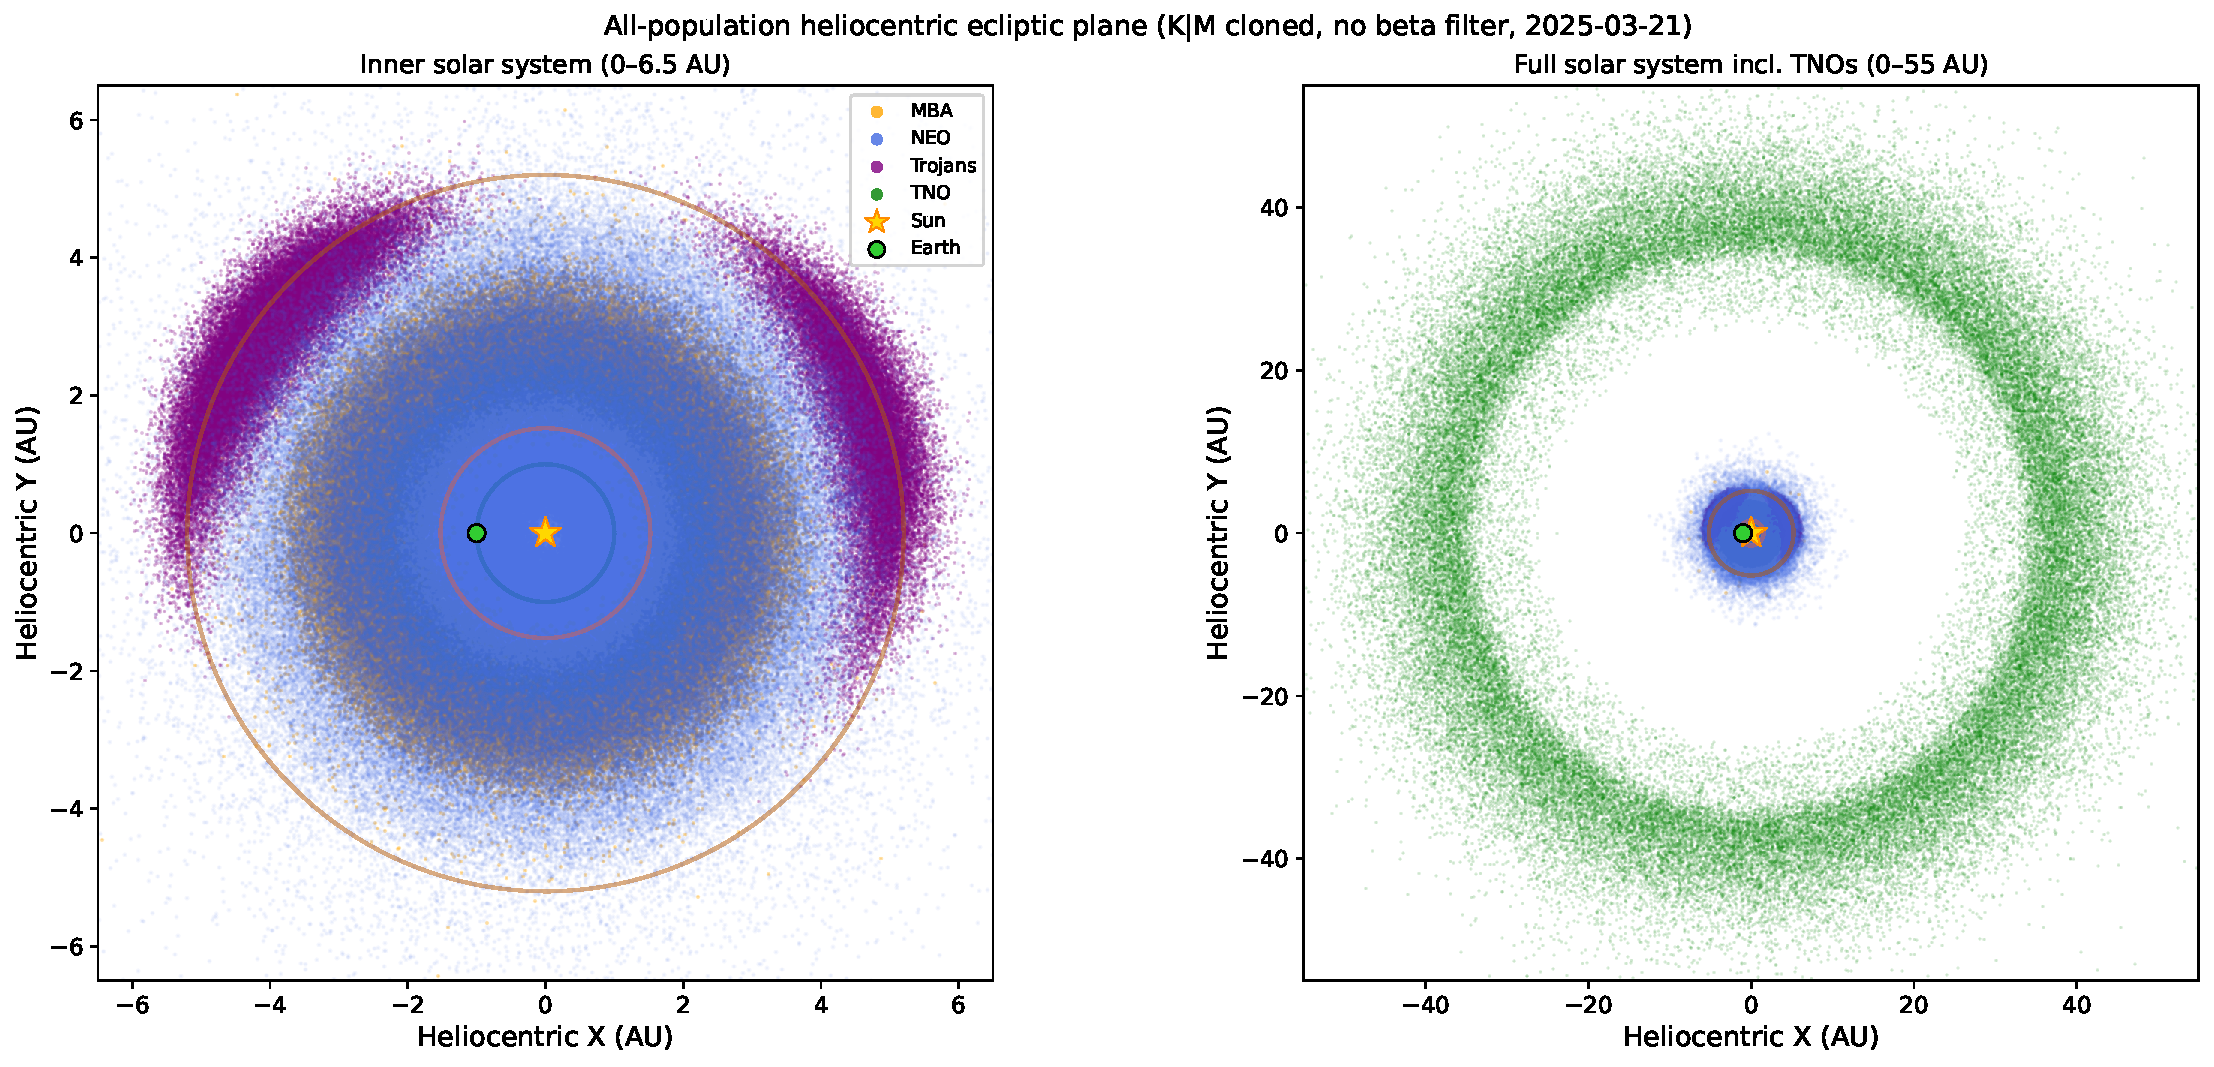
\includegraphics[width=\textwidth]{helio_map_all_populations.png}
\caption{
Heliocentric ecliptic-plane distribution of the four asteroid populations at the Spring Equinox epoch (2025 March 21), projected onto the $X$--$Y$ plane.
\textit{Left:} Inner solar system (0--6.5~au) showing Main Belt Asteroids (MBA, orange), Near-Earth Objects (NEO, blue), and Jupiter Trojans (purple) clustered at the Jovian L4 and L5 Lagrange points.
\textit{Right:} Full solar system (0--55~au) additionally including Trans-Neptunian Objects (TNO, green).
Reference orbit circles for Earth (1.0~au), Mars (1.524~au), and Jupiter (5.203~au) are overplotted.
Positions are derived from K$|$M cloned S3M orbits with no ecliptic latitude filter applied, so the full spatial extent of each population is visible.
}
\label{fig:helio_map}
\end{figure*}


\subsection{Sky-Plane Cuts and Observation Geometry}
\label{sec:compappmag}

We adopt an observation epoch of March 21st 2025, corresponding to the Spring Equinox, and simulate observations in the anti-sun direction which is the point on the sky approximately \( 180^\circ \) opposite to the Sun. This is a good pointing direction for NEO surveys, including LSST, as it places the opposition surge in a favorable location and maximises the sky-plane rates of motion for main-belt objects.

For each population, we apply a series of observability cuts: we restrict objects to within \( \pm 30^\circ \) of the ecliptic plane in ecliptic latitude (\( \beta \)), and examine objects in a series of apparent magnitude bins see Table \ref{tab:mag_bins}. We then construct three-panel diagnostic plots (Figure~\ref{fig:ecliptic_strip_mba_neo}) showing ecliptic longitude ($\lambda$, $0$--$360^\circ$) on the x-axis against ecliptic latitude $\beta$, the rate of motion in longitude ($v_\lambda$, deg/day), and the rate of motion in latitude ($v_\beta$, deg/day) respectively for each population, overlaid to illustrate their relative densities and separability in rate-of-motion space.

\begin{figure*}[ht!]
\centering
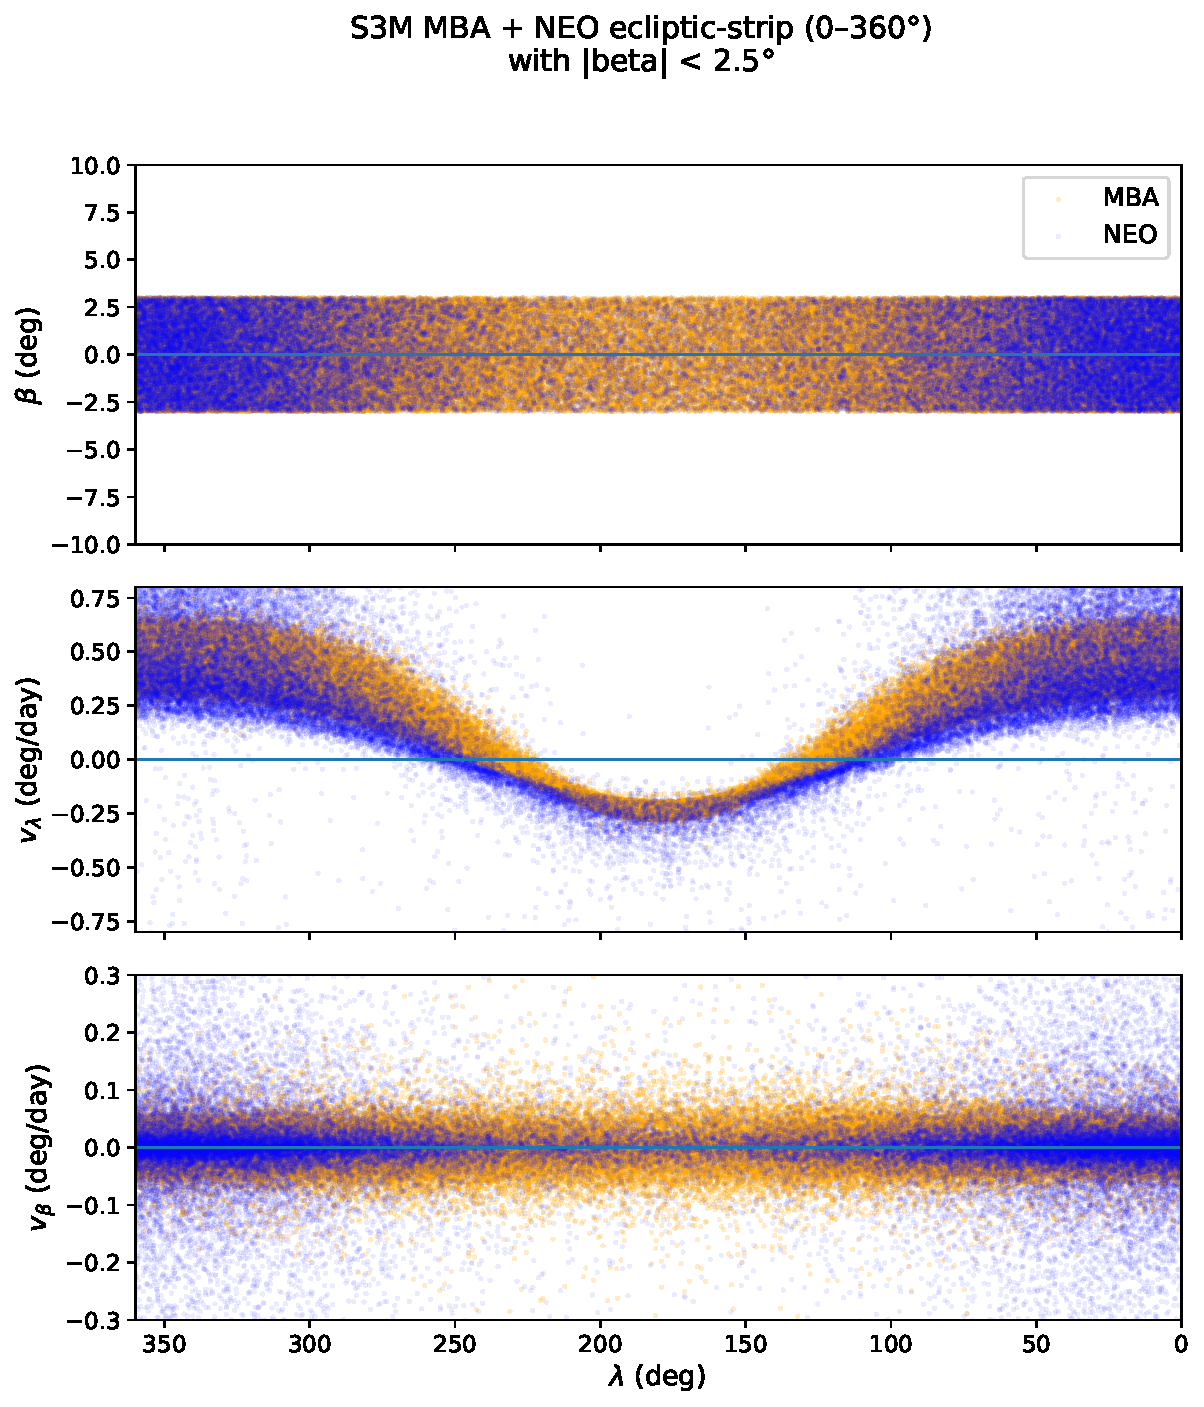
\includegraphics[width=0.75\textwidth]{ecliptic_strip_MBA_NEO.png}
\caption{
Three-panel ecliptic-strip diagnostic for Main Belt Asteroids (MBA, orange) and Near-Earth Objects (NEO, blue) at the Spring Equinox epoch (2025 March 21) with $|\beta| < 3^\circ$, computed using K$|$M cloned orbits from S3M.
\textit{Top:} Ecliptic latitude $\beta$ versus longitude $\lambda$.
\textit{Middle:} Longitudinal rate of motion $v_\lambda$ (deg/day) versus $\lambda$.
\textit{Bottom:} Latitudinal rate of motion $v_\beta$ (deg/day) versus $\lambda$.
The characteristic sinusoidal variation in $v_\lambda$ arises from the anti-solar observing geometry.
MBAs occupy a dense, narrow band near $v_\lambda \approx -0.3$ to $0.0$~deg/day, while NEOs exhibit broader distributions extending to higher velocities, enabling population separation in $v_\lambda$--$v_\beta$ space.
}
\label{fig:ecliptic_strip_mba_neo}
\end{figure*}

These plots confirmed that NEOs and MBAs are significantly separated in \( v_\lambda \)–\( v_\beta \) space, particularly at high rates of motion and large ecliptic latitudes, consistent with the findings of Keys et al. (2019). We also reproduce the characteristic two-clump (L4 and L5) structure of Jupiter Trojans in ecliptic longitude, which serves as an additional validation of the propagation code.

The apparent magnitude is computed using the HG phase-function model,
\begin{equation}
m = H + 5\log_{10}(r\Delta) - 2.5\log_{10}\Phi(\alpha),
\end{equation}
where \(H\) is the absolute magnitude, \(r\) is the heliocentric distance in AU,
\(\Delta\) is the observer-object distance in AU, and \(\alpha\) is the solar
phase angle.

The phase function is
\begin{equation}
\Phi(\alpha) = (1-G)\Phi_1(\alpha) + G\Phi_2(\alpha),
\end{equation}
with
\begin{equation}
\Phi_1(\alpha) =
\exp\left[-A_1\tan^{B_1}\left(\frac{\alpha}{2}\right)\right],
\end{equation}
\begin{equation}
\Phi_2(\alpha) =
\exp\left[-A_2\tan^{B_2}\left(\frac{\alpha}{2}\right)\right].
\end{equation}

We adopt the standard parameter values

\begin{equation}
\begin{aligned}
 G &= 0.15, \\
 A_1 &= 3.33, \\
 A_2 &= 1.87, \\
 B_1 &= 0.63, \\
 B_2 &= 1.22.
\end{aligned}
\end{equation}


\begin{table}[h!]
\centering
\begin{tabular}{lcc}
\hline
\textbf{Label} & \textbf{$m_{\min}$} & \textbf{$m_{\max}$} \\
\hline
14--16  & 14.0 & 16.0 \\
16--18  & 16.0 & 18.0 \\
18--20  & 18.0 & 20.0 \\
20--21  & 20.0 & 21.0 \\
21--22  & 21.0 & 22.0 \\
22--23  & 22.0 & 23.0 \\
23--24  & 23.0 & 24.0 \\
24--26  & 24.0 & 26.0 \\
\hline
\end{tabular}
\caption{Apparent magnitude bins used in this work.}
\label{tab:mag_bins}
\end{table}


\subsection{Population Cloning}
\label{sec:cloneast}

After applying the sky and magnitude cuts described above, we found that the resulting object counts, particularly for NEOs, were too sparse to support a reliable density estimation. To address this, we cloned each population by generating synthetic objects that statistically represent the same orbital family while filling in the phase space more densely.

Our initial approach was to randomise the mean anomaly \( M \) uniformly from \( 0^\circ \) to \( 360^\circ \) for each object. However, this caused the Jupiter Trojans to lose their characteristic L4 and L5 clumping, as uniformly redistributing objects in mean anomaly breaks the resonant structure that confines them near the Lagrange points.

We therefore adopted a more careful approach: for each population subset that survived the sky cuts, we measured the maximum and minimum mean anomaly of the surviving objects, and randomised \( M \) only within that range. Simultaneously, we held the longitude of the ascending node \( \Omega \) fixed and varied the argument of perihelion \( \omega \) in order to preserve the linear relationship with mean longitude. After cloning, we reapplied the \( \pm 30^\circ \) ecliptic latitude cut to ensure that the generated objects remain physically consistent with our observational constraints. This approach successfully reproduced the L4 and L5 Trojan clumps within the correct sky region, confirming that our cloning procedure respects the dynamical structure of each population.

We additionally generated heliocentric Cartesian coordinate plots for each population following the cuts, providing a visual check of the spatial distribution of objects at our chosen epoch.

Quantitative validation of the conditional K$|$M cloner is presented in Section~\ref{sec:clonepop}, including a direct comparison of mean-anomaly distributions for all four populations (Figure~\ref{fig:M_dist}) and a demonstration that the Trojan L4/L5 resonant structure is preserved (Figure~\ref{fig:trojan_l4l5}).



\subsection{How to: propagate your elements once you clone them}
\label{sec:propagation}

The conditional K$|$M cloner (Section~\ref{sec:cloneast}) outputs a new set of Keplerian orbital elements $(a, e, i, \Omega, \omega, t_p)$ for each synthetic clone, where the perihelion time $t_p$ encodes the newly drawn mean anomaly.
Converting these elements into observable sky-plane quantities requires explicit propagation to the observation epoch.

For each clone, we solve Kepler's equation using Newton's method (10 iterations) to obtain the eccentric anomaly $E$ at the observation time $t_\mathrm{obs}$, and thence the heliocentric ecliptic position and velocity vectors $(\mathbf{r}_\mathrm{ecl}, \dot{\mathbf{r}}_\mathrm{ecl})$.
These are rotated from ecliptic to equatorial coordinates using the obliquity $\varepsilon = 23.439^\circ$, and the observer's heliocentric state (Earth + topocentric offset) is subtracted to form the topocentric position $\mathbf{\rho}$ and velocity $\dot{\mathbf{\rho}}$.
Right ascension, declination, and their time derivatives follow directly from $\mathbf{\rho}$ and $\dot{\mathbf{\rho}}$; the ecliptic rates $(v_\lambda, v_\beta)$ are obtained by rotating the position and velocity unit vectors back to the ecliptic frame via the obliquity matrix.
We perform this rotation analytically rather than through the \texttt{astropy} \texttt{GeocentricTrueEcliptic} coordinate transform, which does not preserve velocity differentials and would discard $\dot{v}_\lambda$ and $\dot{v}_\beta$.

After propagation, the same $30^\circ$ sky-patch cut is reapplied to the full cloned sample, retaining only the synthetic objects that fall within the observational footprint at the chosen epoch.
This ``clone then cut'' order is essential: generating $\mathrm{clone\_factor}$ times more orbits before the sky cut ensures adequate density across the velocity grid even in sparsely populated dynamical regions.


\subsection{Validation and Characteristics of Cloned Population}
\label{sec:clonepop}

We validate the conditional K$|$M cloner on three independent grounds: (1) recovery of the empirical mean-anomaly distribution, (2) preservation of the Jupiter Trojan L4/L5 resonant structure, and (3) physically consistent ecliptic-strip diagnostics for all four populations.

\subsubsection*{Mean-anomaly distribution recovery}

The defining property of the conditional K$|$M cloner is that it draws new mean anomalies $M$ from the \emph{empirical} distribution of the surviving visible objects, rather than imposing uniformity.
Figure~\ref{fig:M_dist} shows, for each population, the distribution of $M$ in the raw S3M catalogue (blue) alongside the distribution recovered by the cloner (orange dashed).
In all four cases the cloned distribution tracks the input, including population-specific features such as the bimodal structure of the Trojan sample and the mild non-uniformity present in the MBA and NEO distributions at the chosen epoch.
A uniform-$M$ cloner would flatten these distributions by construction, introducing a systematic mismatch between the cloned and real orbital phase populations.

\begin{figure*}[ht!]
\centering
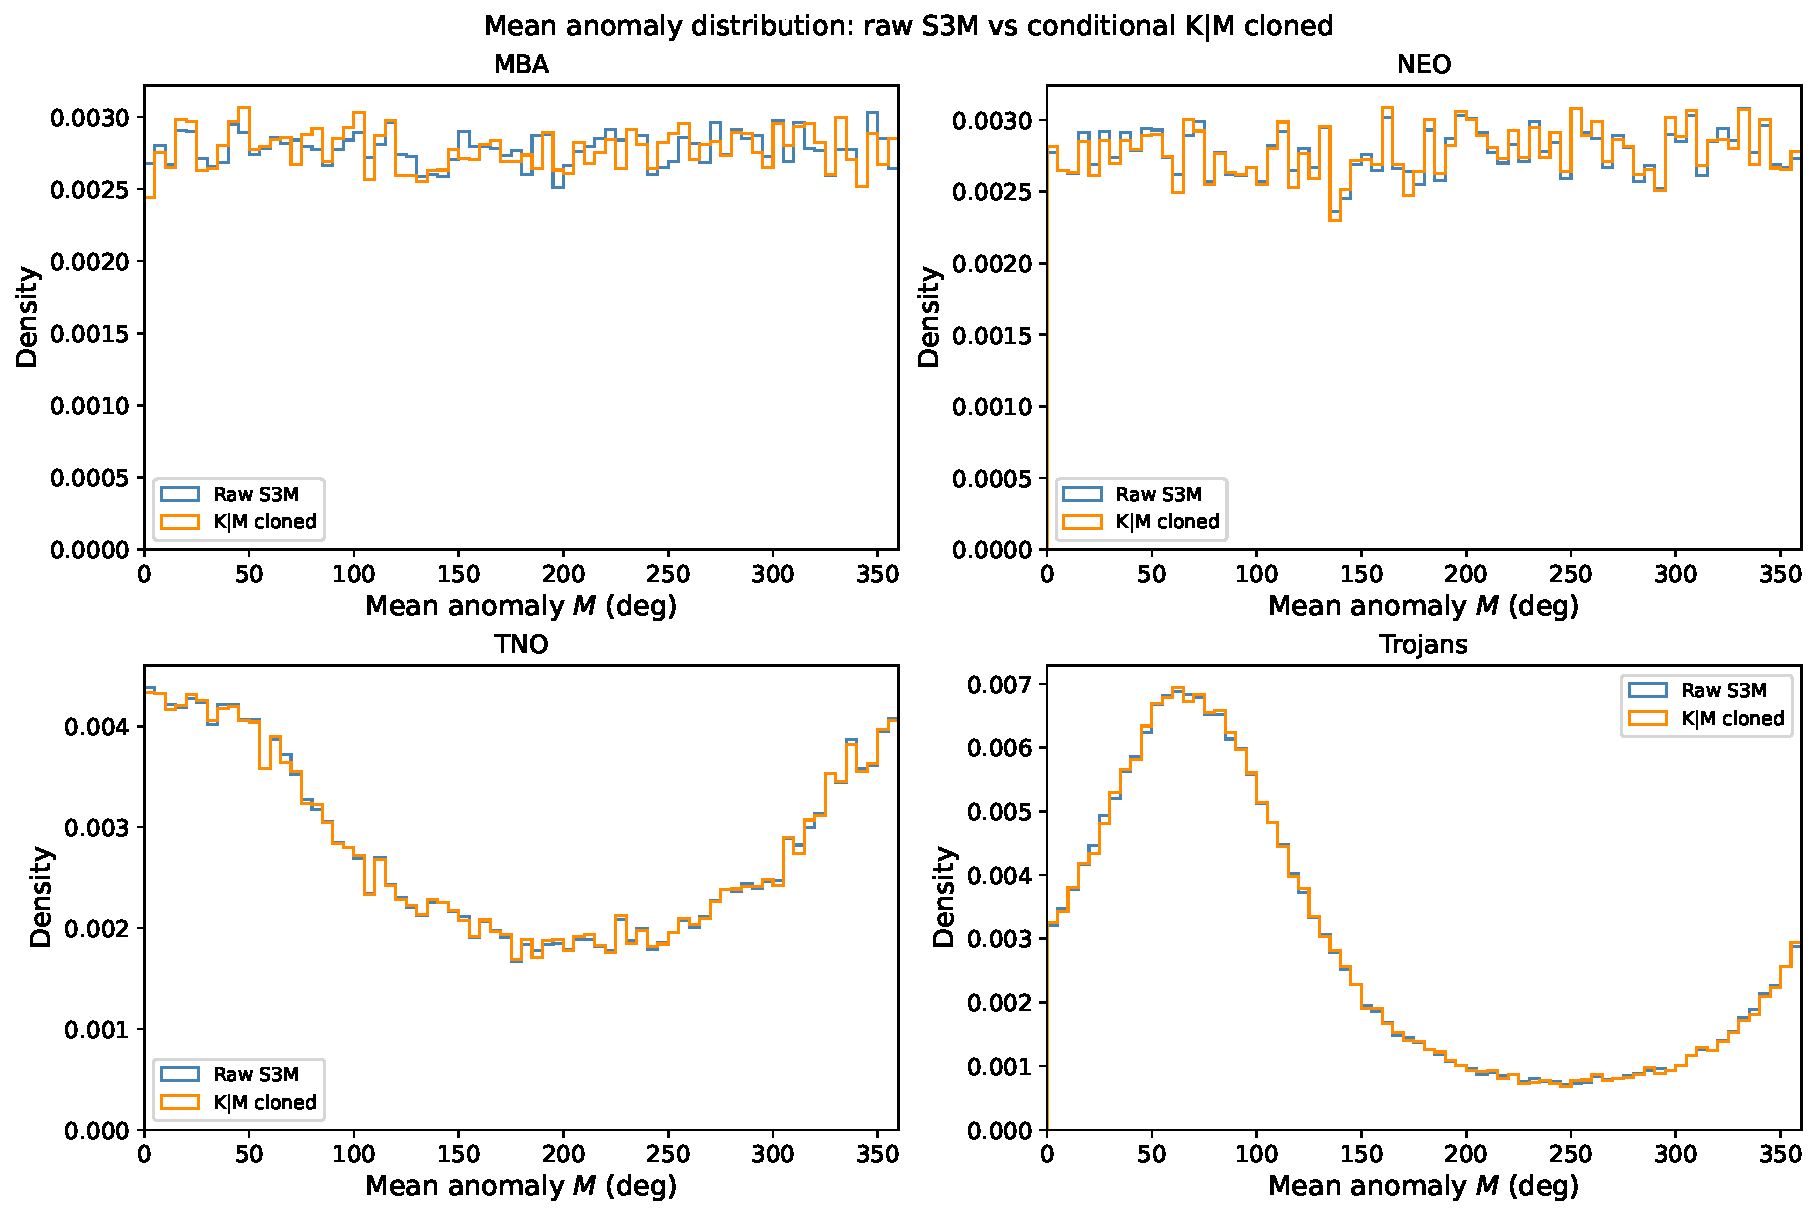
\includegraphics[width=0.85\textwidth]{comparison_M_distribution.png}
\caption{
Comparison of mean anomaly $M$ distributions between raw S3M objects (blue) and K$|$M cloned objects (orange dashed) for each of the four asteroid populations.
In all cases the conditional cloner reproduces the empirical $M$ distribution of the visible input sample rather than imposing uniformity, confirming that the cloning procedure does not introduce artificial biases in orbital phase.
}
\label{fig:M_dist}
\end{figure*}

\subsubsection*{Jupiter Trojan L4/L5 preservation}

The most sensitive test of the cloner is the Jupiter Trojan population, whose objects are gravitationally confined to the L4 and L5 Lagrange points and consequently concentrated near mean longitudes $\mathcal{L} = M + \Omega + \omega \approx 60^\circ$ and $300^\circ$ relative to Jupiter.
Figure~\ref{fig:trojan_l4l5} compares the mean-longitude distribution of Trojans under three scenarios: the raw S3M catalogue, naive uniform-$M$ randomisation, and the conditional K$|$M cloner.
Uniform-$M$ randomisation completely destroys the L4/L5 double-clump structure by redistributing objects uniformly across all orbital phases; the resulting velocity-space density maps would misrepresent Trojan kinematics wherever their sky-plane rate distribution depends on orbital phase.
The K$|$M cloner, by contrast, reproduces both clumps at the correct mean longitudes, confirming that the resonant structure is preserved through the cloning step.

\begin{figure*}[ht!]
\centering
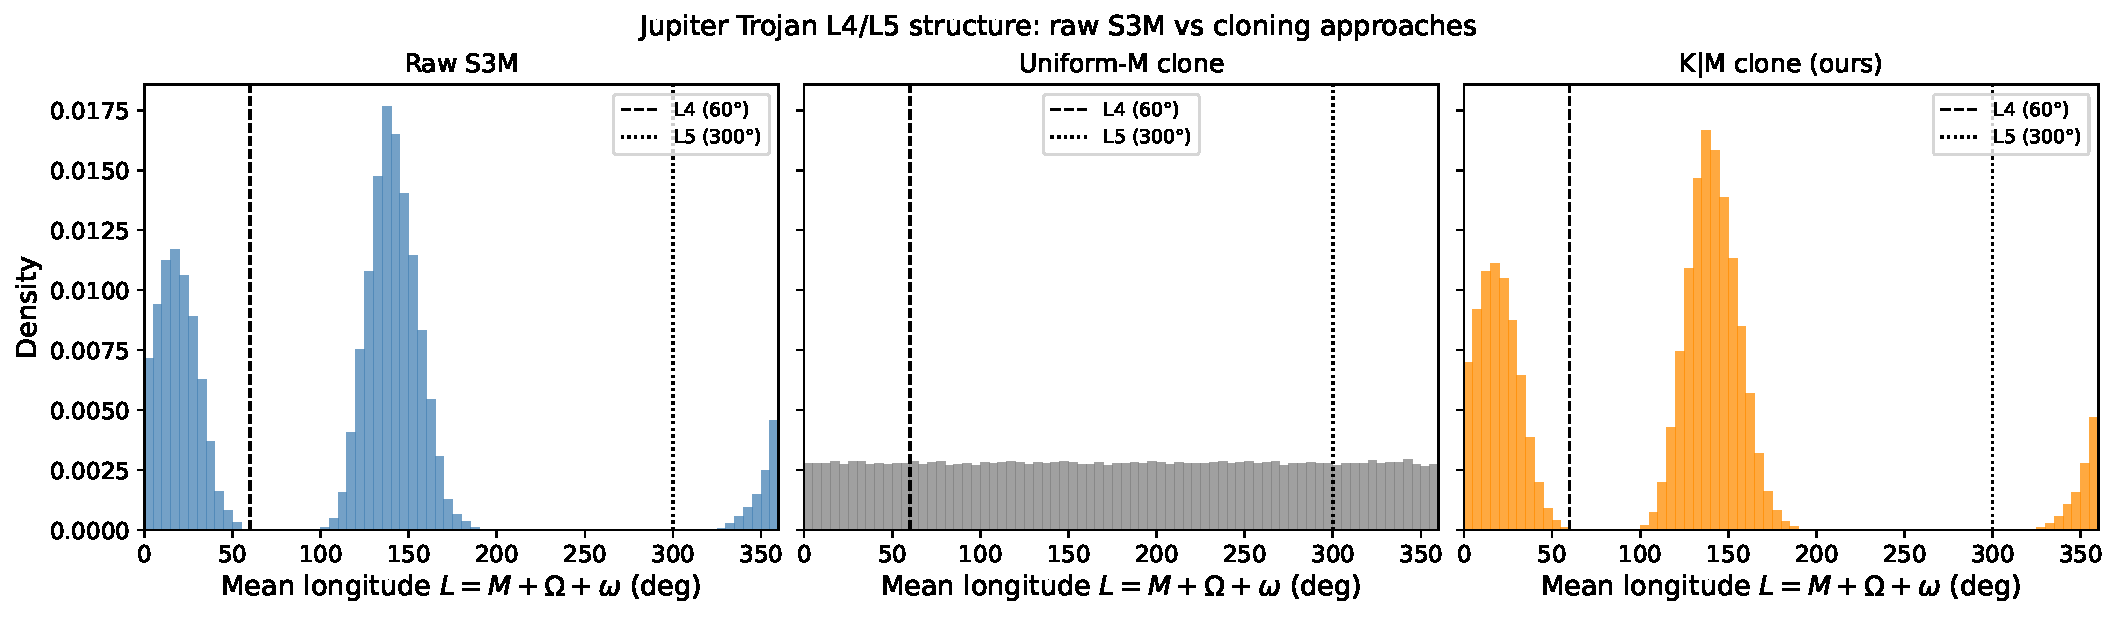
\includegraphics[width=\textwidth]{trojan_L4L5_comparison.png}
\caption{
Jupiter Trojan L4/L5 clump preservation under three cloning approaches, showing the distribution of mean longitude $\mathcal{L} = M + \Omega + \omega$.
\textit{Left:} Raw S3M catalogue, exhibiting the two characteristic clumps near the Jovian L4 ($60^\circ$) and L5 ($300^\circ$) Lagrange points (dashed lines).
\textit{Centre:} Naive uniform-$M$ randomisation, which destroys the clump structure by redistributing objects uniformly across all orbital phases.
\textit{Right:} Conditional K$|$M cloning (this work), which preserves the empirical mean-anomaly distribution of the surviving objects, successfully reproducing the L4/L5 double-clump structure.
}
\label{fig:trojan_l4l5}
\end{figure*}

\subsubsection{Ecliptic-strip diagnostics for all populations}
\label{sec:eclipticstrip}

The ecliptic-strip pipeline propagates each cloned orbit to the observation epoch using Kepler's equation, transforms to geocentric ecliptic coordinates, and computes the sky-plane rates of motion $v_\lambda$ and $v_\beta$ from the ecliptic velocity components.
Figure~\ref{fig:ecliptic_strip_mba_neo} (Section~\ref{sec:compappmag}) shows this for the MBA and NEO populations.
Figures~\ref{fig:ecliptic_strip_trojans} and~\ref{fig:ecliptic_strip_tno} extend the same diagnostic to Jupiter Trojans and TNOs respectively, confirming that the K$|$M cloner reproduces the expected dynamical structure of each population.

\begin{figure*}[ht!]
\centering
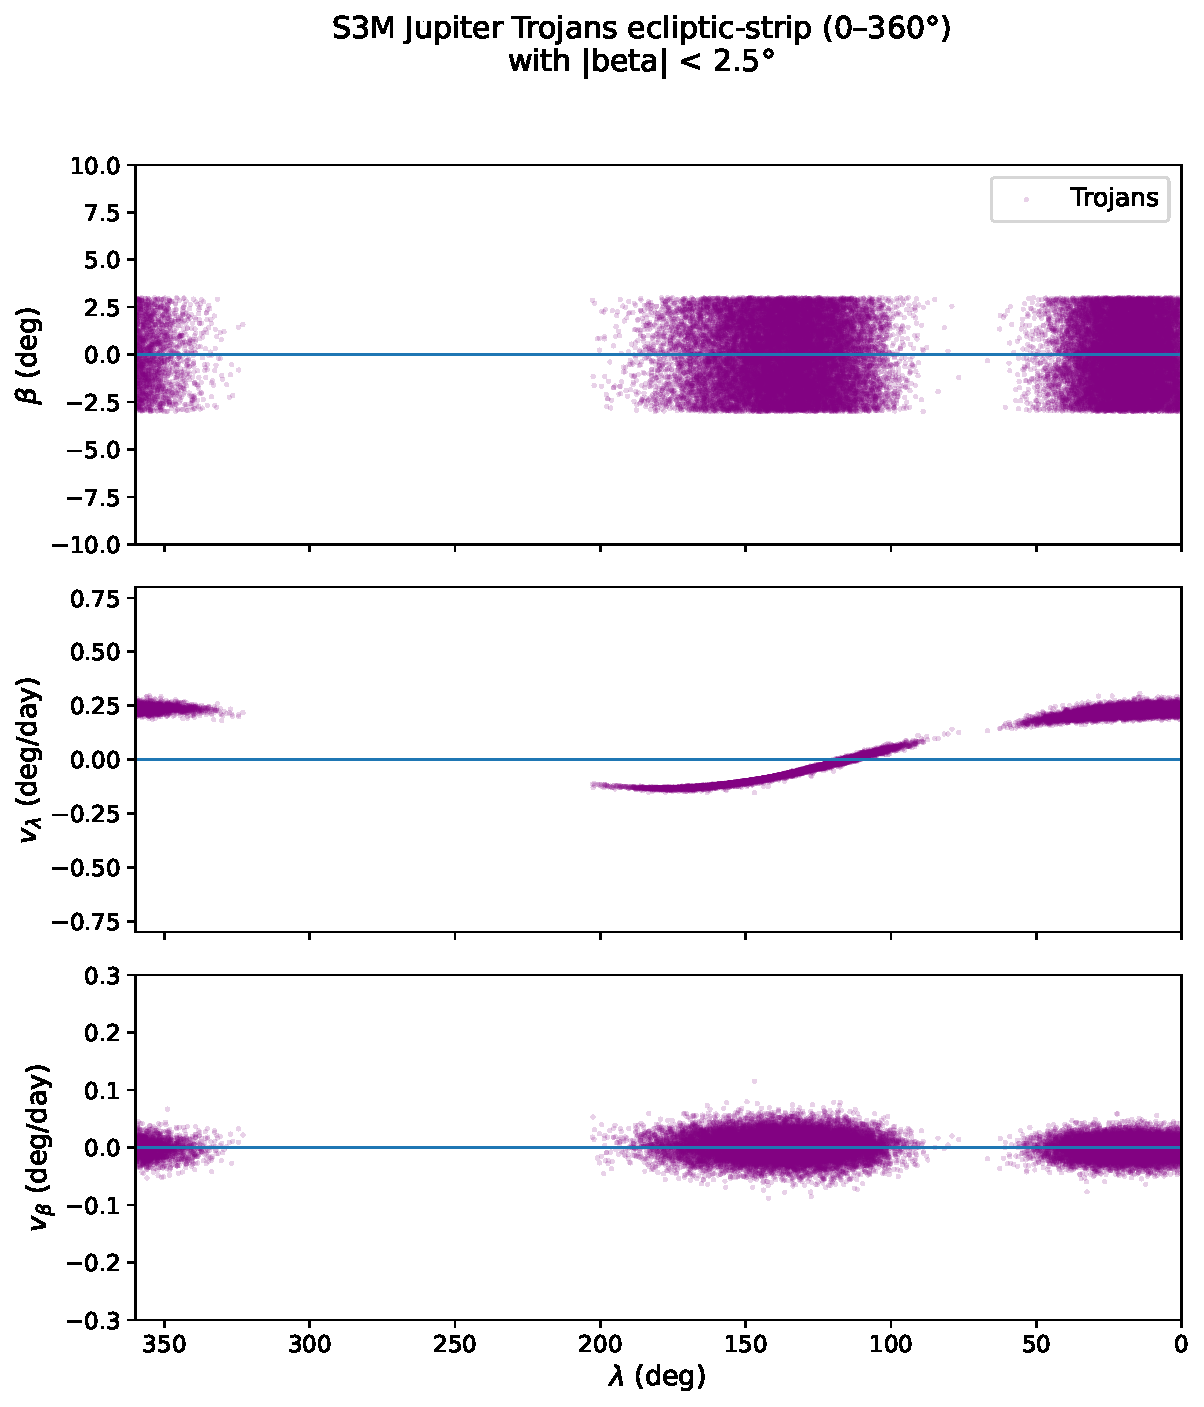
\includegraphics[width=0.75\textwidth]{ecliptic_strip_Trojans.png}
\caption{
Three-panel ecliptic-strip diagnostic for Jupiter Trojans at the Spring Equinox epoch (2025 March 21) with $|\beta| < 3^\circ$, using K$|$M cloned orbits.
The two distinct clumps correspond to the L4 (leading, $\lambda \approx 300^\circ$ in the anti-solar frame) and L5 (trailing, $\lambda \approx 60^\circ$) populations.
The narrow range in both $v_\lambda$ and $v_\beta$ reflects the Trojans' near-circular orbits co-rotating with Jupiter at 5.2~au.
}
\label{fig:ecliptic_strip_trojans}
\end{figure*}

\begin{figure*}[ht!]
\centering
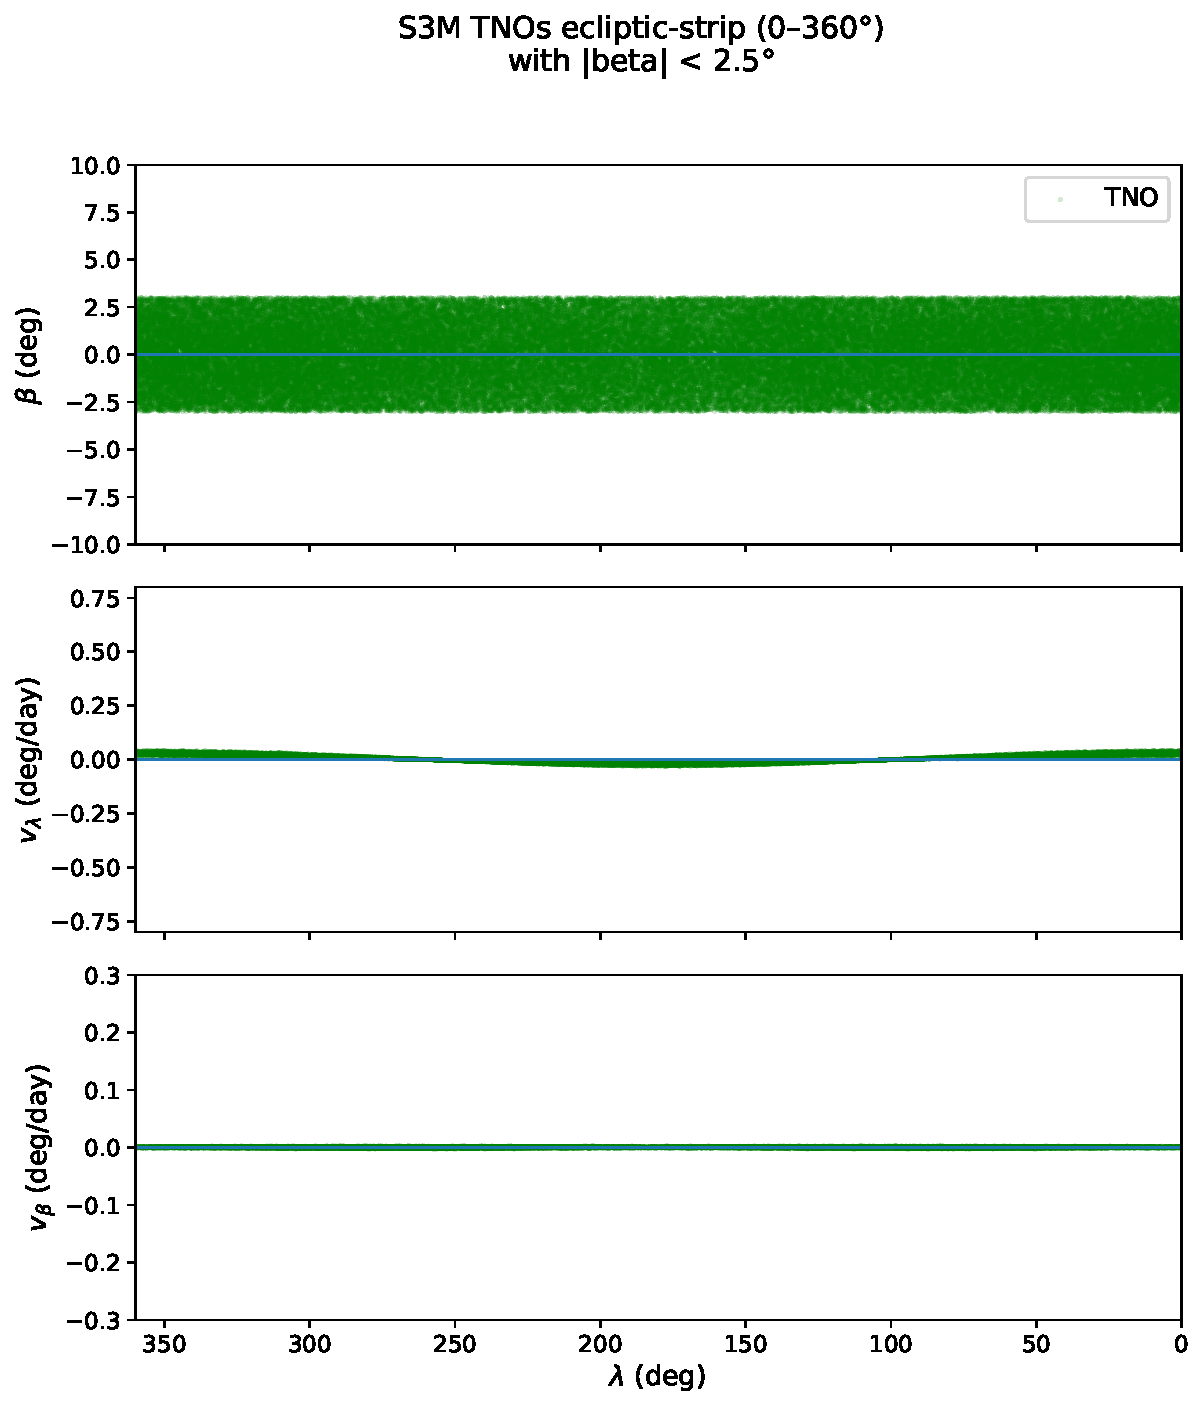
\includegraphics[width=0.75\textwidth]{ecliptic_strip_TNO.png}
\caption{
Three-panel ecliptic-strip diagnostic for Trans-Neptunian Objects (TNOs) at the Spring Equinox epoch (2025 March 21) with $|\beta| < 3^\circ$, using K$|$M cloned orbits.
TNOs cluster near $v_\lambda \approx v_\beta \approx 0$~deg/day across all ecliptic longitudes, reflecting their large heliocentric distances (30--100~au) which produce extremely slow apparent sky-plane velocities relative to the inner-belt populations.
}
\label{fig:ecliptic_strip_tno}
\end{figure*}


\subsection{Bayesian Density Estimation and Probability Maps}
\label{sec:bayesian}

With the cloned populations propagated and visible subsets selected, we estimate the local number density of each population across a uniform $161 \times 161$ grid in $(v_\lambda, v_\beta)$ space, spanning $[-0.8, +0.8]$~deg/day in each axis at a spacing of $0.01$~deg/day (25,921 evaluation points total).
We use the self-adaptive Bayesian nearest-neighbour density estimator of Appendix~B of \citet{Ivezic2001}, which requires no fixed bandwidth and naturally provides finer resolution in crowded regions (e.g.\ the MBA clump) and coarser smoothing where objects are sparse (e.g.\ the NEO high-velocity tail).

\subsubsection*{Density estimation}

At each grid point $\mathbf{q} = (v_\lambda, v_\beta)$, we query a pre-built \texttt{cKDTree} of the cloned sample for the $k = 5$ nearest-neighbour distances $d_1 \leq d_2 \leq \cdots \leq d_k$.
Under the assumption that the local population is approximately uniform with 2D number density $n_0$, the $j$-th order-statistic distance follows the distribution
\begin{equation}
  p(d_j \mid n_0) = \frac{2}{\sigma_0} \left(\frac{d_j}{\sigma_0}\right)^{2j-1}
  \frac{\exp[-(d_j/\sigma_0)^2]}{\Gamma(j)},
  \quad \sigma_0 \equiv \frac{1}{\sqrt{\pi n_0}}.
\end{equation}
Treating $n_0$ as unknown and placing a flat prior on the characteristic scale $\sigma_0$, the unnormalized log-posterior of $\sigma_0$ given all $k$ distances is
\begin{equation}
  \log p(\sigma_0 \mid d_1,\ldots,d_k)
  = \sum_{j=1}^{k}
    \left[\log 2 - \log \sigma_0 - \log\Gamma(j)
    - \left(\frac{d_j}{\sigma_0}\right)^2
    + (2j-1)\log\frac{d_j}{\sigma_0}\right].
\end{equation}
This is evaluated on a logarithmically-spaced grid of 400 trial values of $\sigma_0$, normalized by the trapezoid rule (with a log-shift for numerical stability), and used to compute the posterior-mean local density
\begin{equation}
  \langle n_0 \rangle = \int_0^\infty \frac{1}{\pi \sigma_0^2}\, p(\sigma_0 \mid \mathbf{d})\, \mathrm{d}\sigma_0.
\end{equation}
The resulting $\langle n_0 \rangle$ is our density estimate at $\mathbf{q}$; the full map is assembled by looping this estimator over all 25,921 grid points.
Each per-population map is then divided by the clone factor used for that population to restore the normalisation to the equivalent un-cloned sample density.

\subsubsection*{Probability maps and the velocity mask}

Population membership probabilities follow from the normalised ratio
\begin{equation}
  P(\mathrm{pop} \mid v_\lambda, v_\beta)
  = \frac{\rho_{\mathrm{pop}}(v_\lambda, v_\beta)}
         {\displaystyle\sum_{\mathrm{pops}} \rho_{\mathrm{pop}}(v_\lambda, v_\beta)},
\end{equation}
where $\rho_{\mathrm{pop}}$ denotes the downweighted posterior-mean density map for a given population.
Because the kNN estimator returns small but finite values everywhere (it never returns exactly zero), we additionally impose a nearest-object mask: any grid cell whose nearest cloned object exceeds $r_\mathrm{mask} = 0.2$~deg/day is set to zero probability.
This mask suppresses probability in velocity regions that are genuinely unsampled by the cloned catalogue, rather than merely low-density; it appears as the sharp outer boundary visible in the probability maps (Figures~\ref{fig:density_bins} and~\ref{fig:prob_bins}).

\subsection{Velocity-space density and probability maps by magnitude}
\label{sec:magbinmaps}

With the cloned populations constructed, we compute density maps in $v_\lambda$--$v_\beta$ space separately for each apparent magnitude bin (Table~\ref{tab:mag_bins}).
Restricting to a magnitude bin selects the subset of the cloned population that a survey at that depth would observe, which changes the relative population fractions substantially: at bright magnitudes ($m < 18$) the MBA population dominates and NEOs are sparse; at faint magnitudes ($m > 24$) TNOs emerge prominently near zero sky-plane velocity.

Figures~\ref{fig:density_bins} and~\ref{fig:prob_bins} show, for three representative bins, the log-density maps and the derived population membership probability maps respectively.

\begin{figure*}[ht!]
\centering
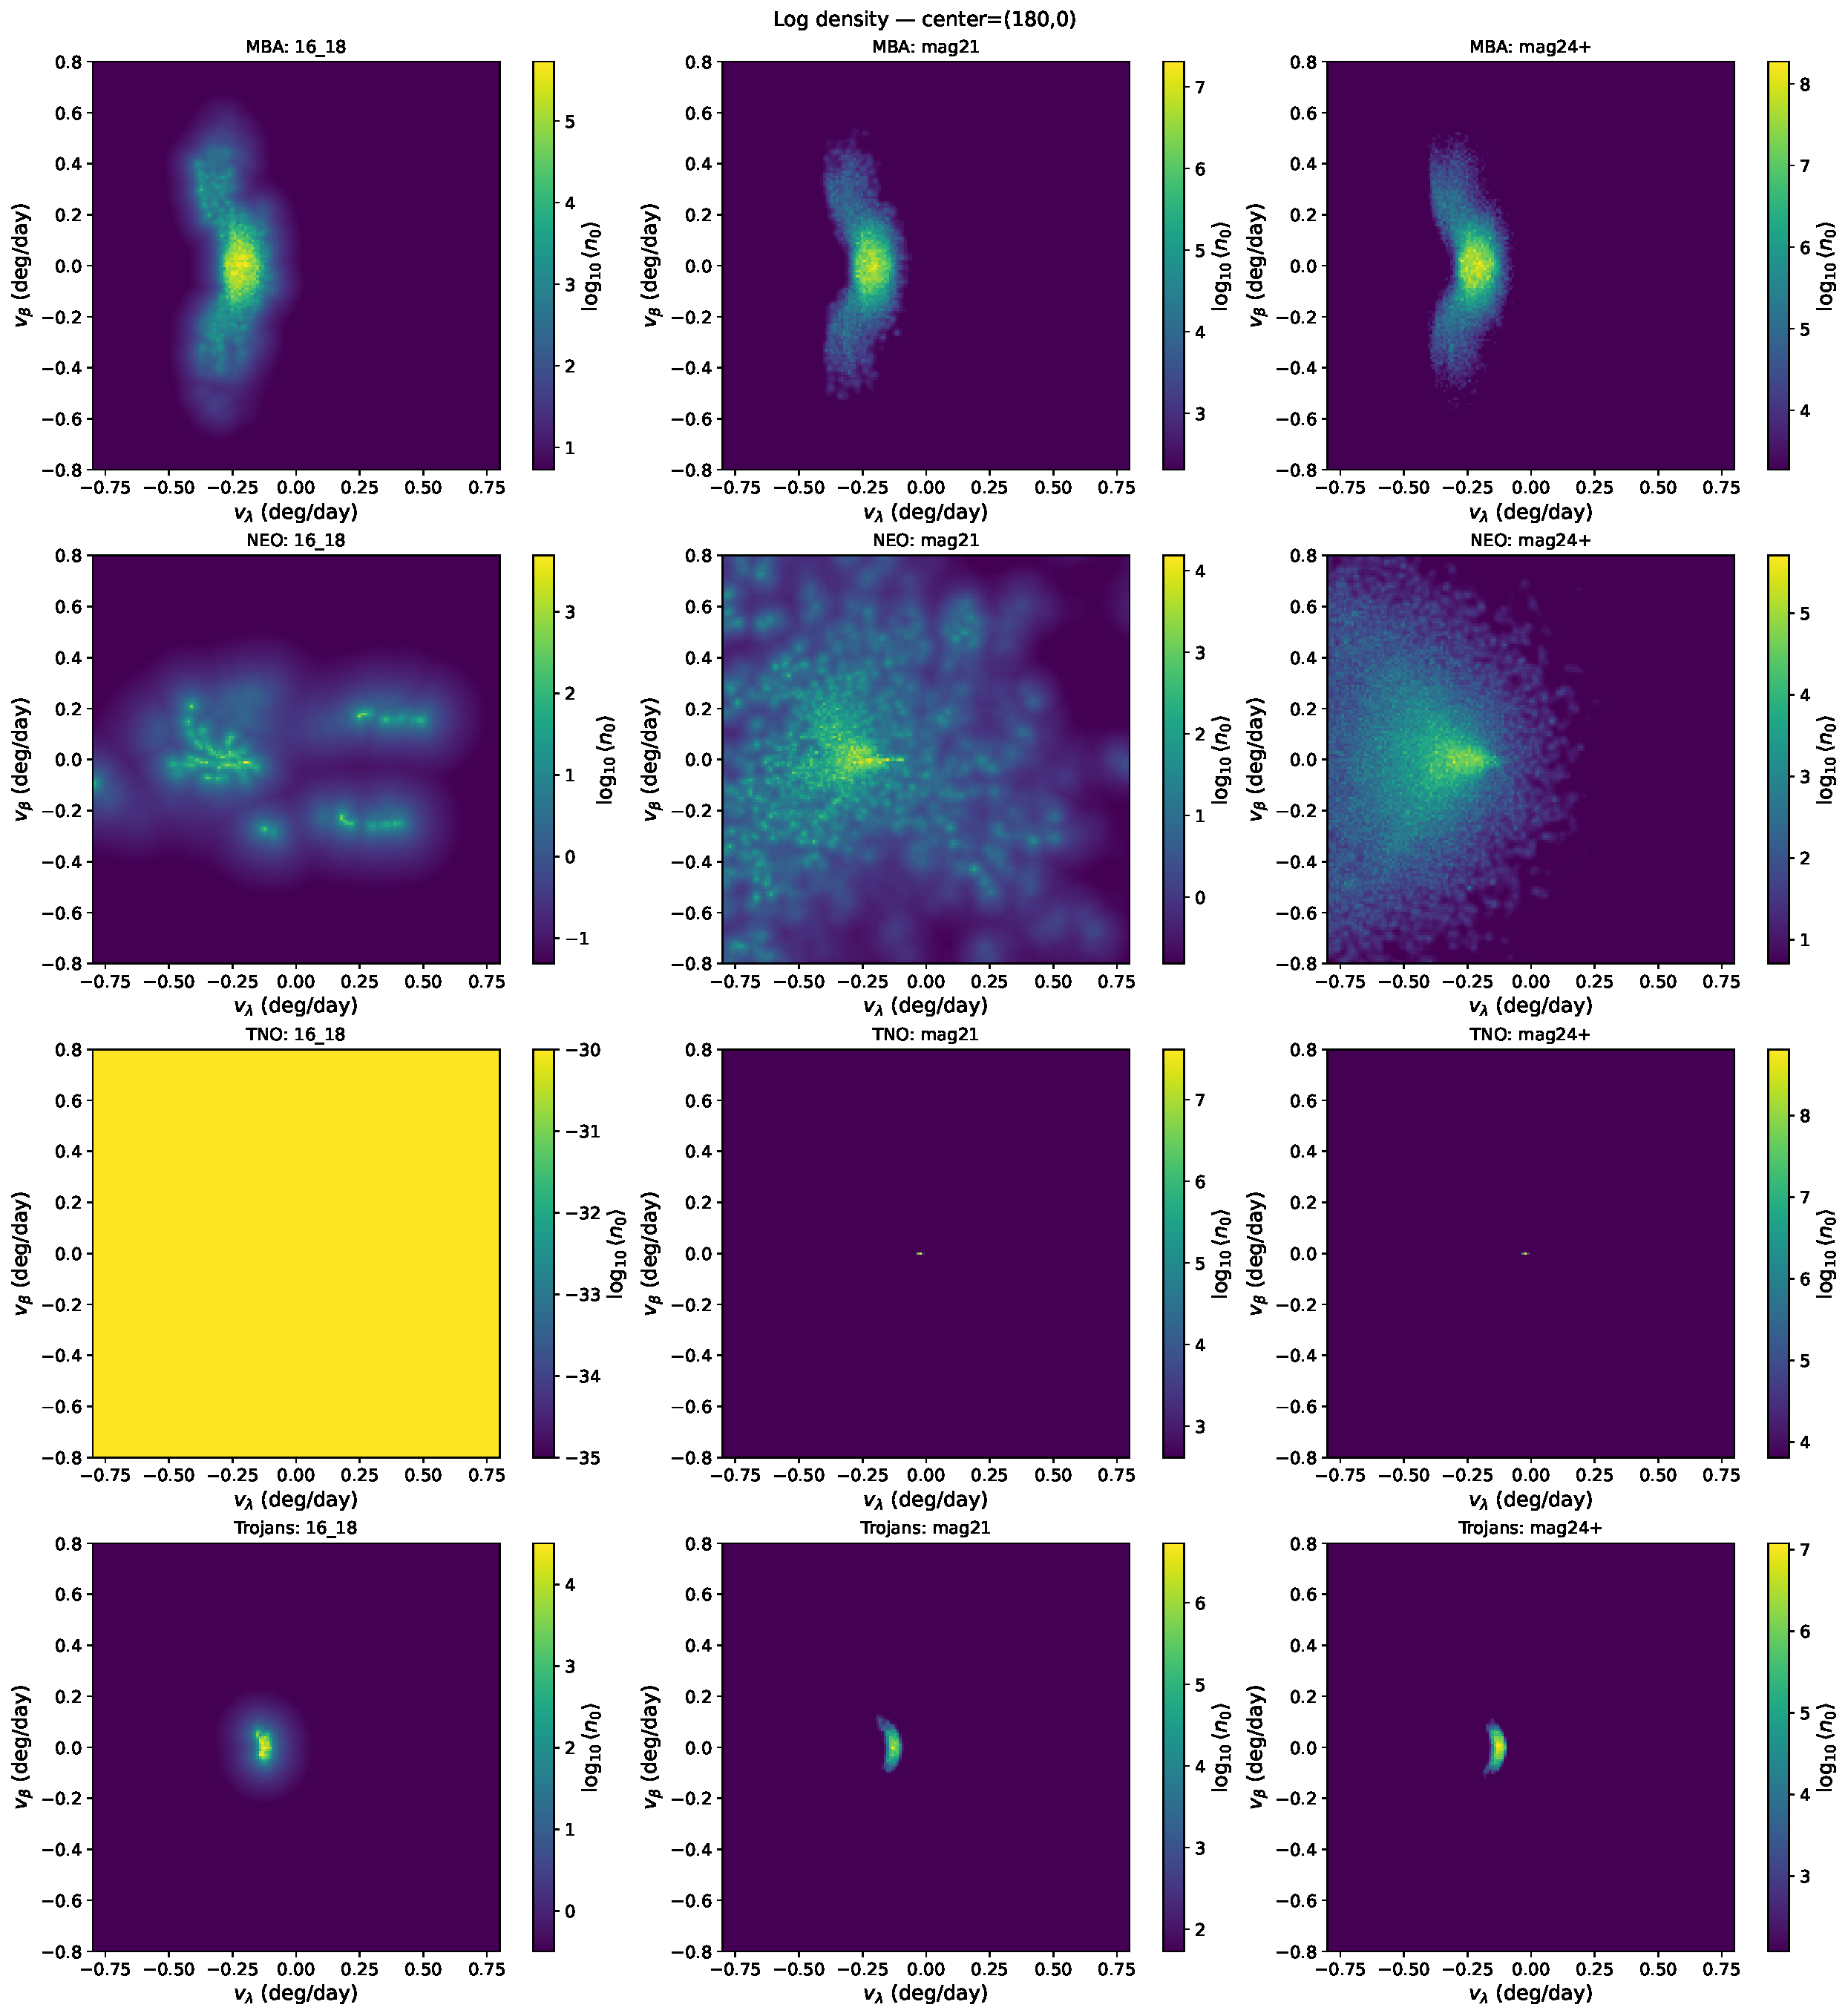
\includegraphics[width=\textwidth]{density_comparison_three_bins.png}
\caption{
Velocity-space log-density maps ($v_\lambda$--$v_\beta$) for the four asteroid populations across three representative apparent magnitude bins: $m \in [16, 18]$ (\textit{left}), $m \in [21, 22]$ (\textit{centre}), and $m \geq 24$ (\textit{right}).
Colour shows $\log_{10}\langle n_0 \rangle$, the kNN posterior-mean density within a 5-decade dynamic range below each panel's peak; regions more than five decades below the peak appear black.
Maps are evaluated at anti-solar pointing (ecliptic lon $= 180^\circ$, lat $= 0^\circ$) at the Spring Equinox epoch.
The MBA distribution (top row) dominates at all magnitudes but narrows as fainter bins favour more distant objects with slower apparent velocities.
TNOs (third row) are undetectable at bright magnitudes but emerge prominently at $m \geq 24$, entirely occupying the near-zero velocity region.
}
\label{fig:density_bins}
\end{figure*}

\begin{figure*}[ht!]
\centering
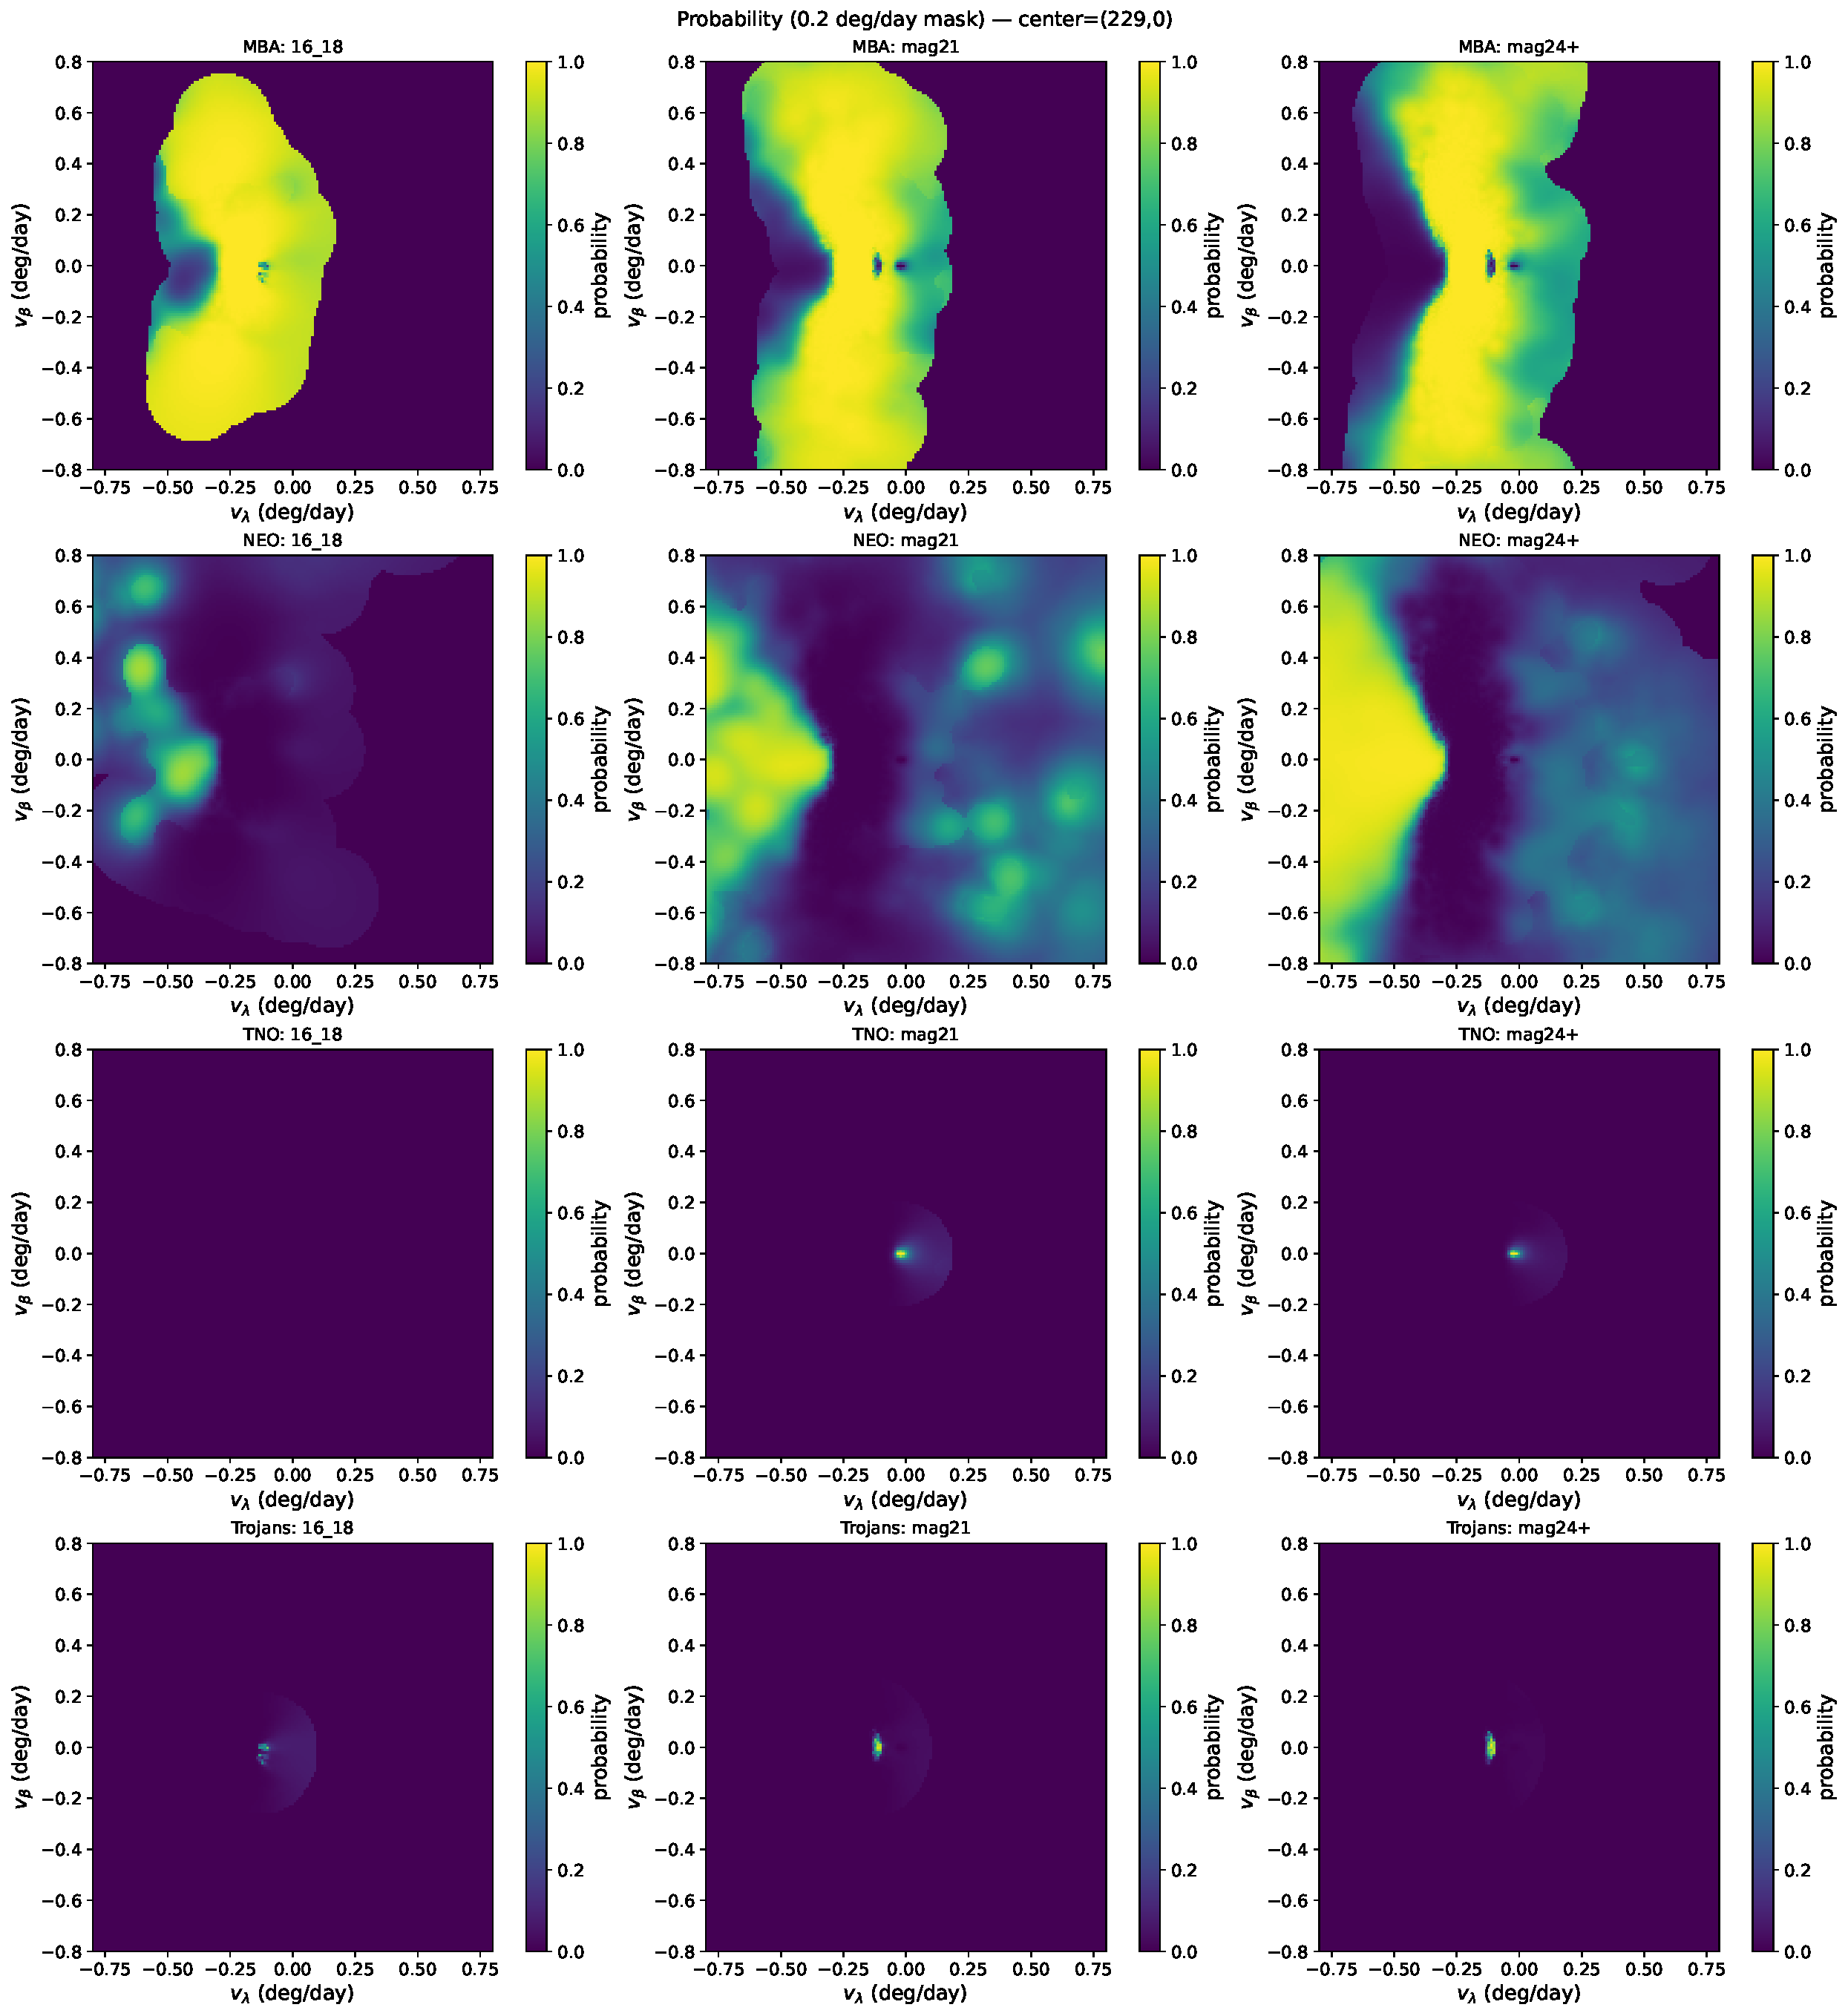
\includegraphics[width=\textwidth]{probability_comparison_three_bins.png}
\caption{
Population membership probability maps in $v_\lambda$--$v_\beta$ space for the four asteroid populations across three representative apparent magnitude bins: $m \in [16, 18]$ (\textit{left}), $m \in [21, 22]$ (\textit{centre}), and $m \geq 24$ (\textit{right}).
The probability is $P(\mathrm{pop} \mid v_\lambda, v_\beta) = \rho_\mathrm{pop} / \sum_\mathrm{pops} \rho_\mathrm{pop}$, masked to zero wherever the nearest cloned object exceeds 0.2~deg/day (unsampled velocity space).
At bright magnitudes, MBAs dominate the slow-motion regime ($v_\lambda \lesssim 0$~deg/day) and NEOs claim the faster-motion wings.
At $m \geq 24$, TNOs reclaim the near-zero velocity region entirely, and the MBA NEO boundary shifts to higher speeds as the faint-magnitude MBA population thins.
These maps form the lookup table used by the classifier at runtime.
}
\label{fig:prob_bins}
\end{figure*}

\subsection{Classifier Evaluation and ROC Analysis}
\label{sec:ROC}

\subsubsection*{Scoring the S3M sample}

To evaluate classifier performance, we propagate all four S3M populations to the observation epoch (2025 March 21) and apply the same $30^\circ$ sky-patch cut used to build the probability maps.
For each surviving object we compute its apparent magnitude (Section~\ref{sec:compappmag}), assign it to the appropriate magnitude bin (Table~\ref{tab:mag_bins}), and look up $P(\mathrm{NEO})$ from the corresponding probability map via bilinear interpolation.
This yields a scored sample of 1,454,634 objects: 1,410,105 MBAs, 23,605 Trojans, 13,497 NEOs, and 7,427 TNOs.
Objects whose apparent magnitude falls outside all defined bins, or whose velocity falls outside the 0.2~deg/day nearest-object mask, receive $P(\mathrm{NEO}) = 0$.

\subsubsection*{ROC curve construction}

We define a binary classifier: call an object a NEO candidate if $P(\mathrm{NEO}) > x$ for a tunable threshold $x \in [0, 1]$.
Sweeping $x$ across 1001 uniformly spaced values, we compute at each threshold
\begin{align}
  \text{Completeness}(x) &= \frac{N_\mathrm{cand}^\mathrm{NEO}(x)}{N_\mathrm{true}^\mathrm{NEO}}, \\
  \text{Contamination}(x) &= \frac{N_\mathrm{cand}^\mathrm{non\text{-}NEO}(x)}
                                   {N_\mathrm{cand}^\mathrm{NEO}(x) + N_\mathrm{cand}^\mathrm{non\text{-}NEO}(x)}.
\end{align}
Plotting completeness against contamination as $x$ varies traces out the Receiver Operating Characteristic (ROC) curve shown in Figure~\ref{fig:roc_curve}.
The optimal operating point $x^*$ is selected by maximising the F1-score, which weights completeness and purity equally.

\subsubsection*{Results}

At the optimal threshold $x^* = 0.137$, the classifier recovers 1,565 true NEOs out of 13,497 ($11.6\%$ completeness) with 805 false positives, giving a purity of $66.0\%$ and a contamination of $34.0\%$.
All false positives at this threshold are MBAs; no Trojans or TNOs pass the cut.
The low absolute completeness reflects the conservative velocity mask: roughly $83\%$ of NEOs visible in the sky patch have $P(\mathrm{NEO}) = 0$ because they fall within the MBA-dominated region of $(v_\lambda, v_\beta)$ space and are therefore indistinguishable from MBAs on the basis of sky-plane motion alone.
The classifier is most powerful for high-rate NEOs and those at large ecliptic latitudes, precisely the objects that are genuinely identifiable from a single-night tracklet.

\begin{figure*}[ht!]
\centering
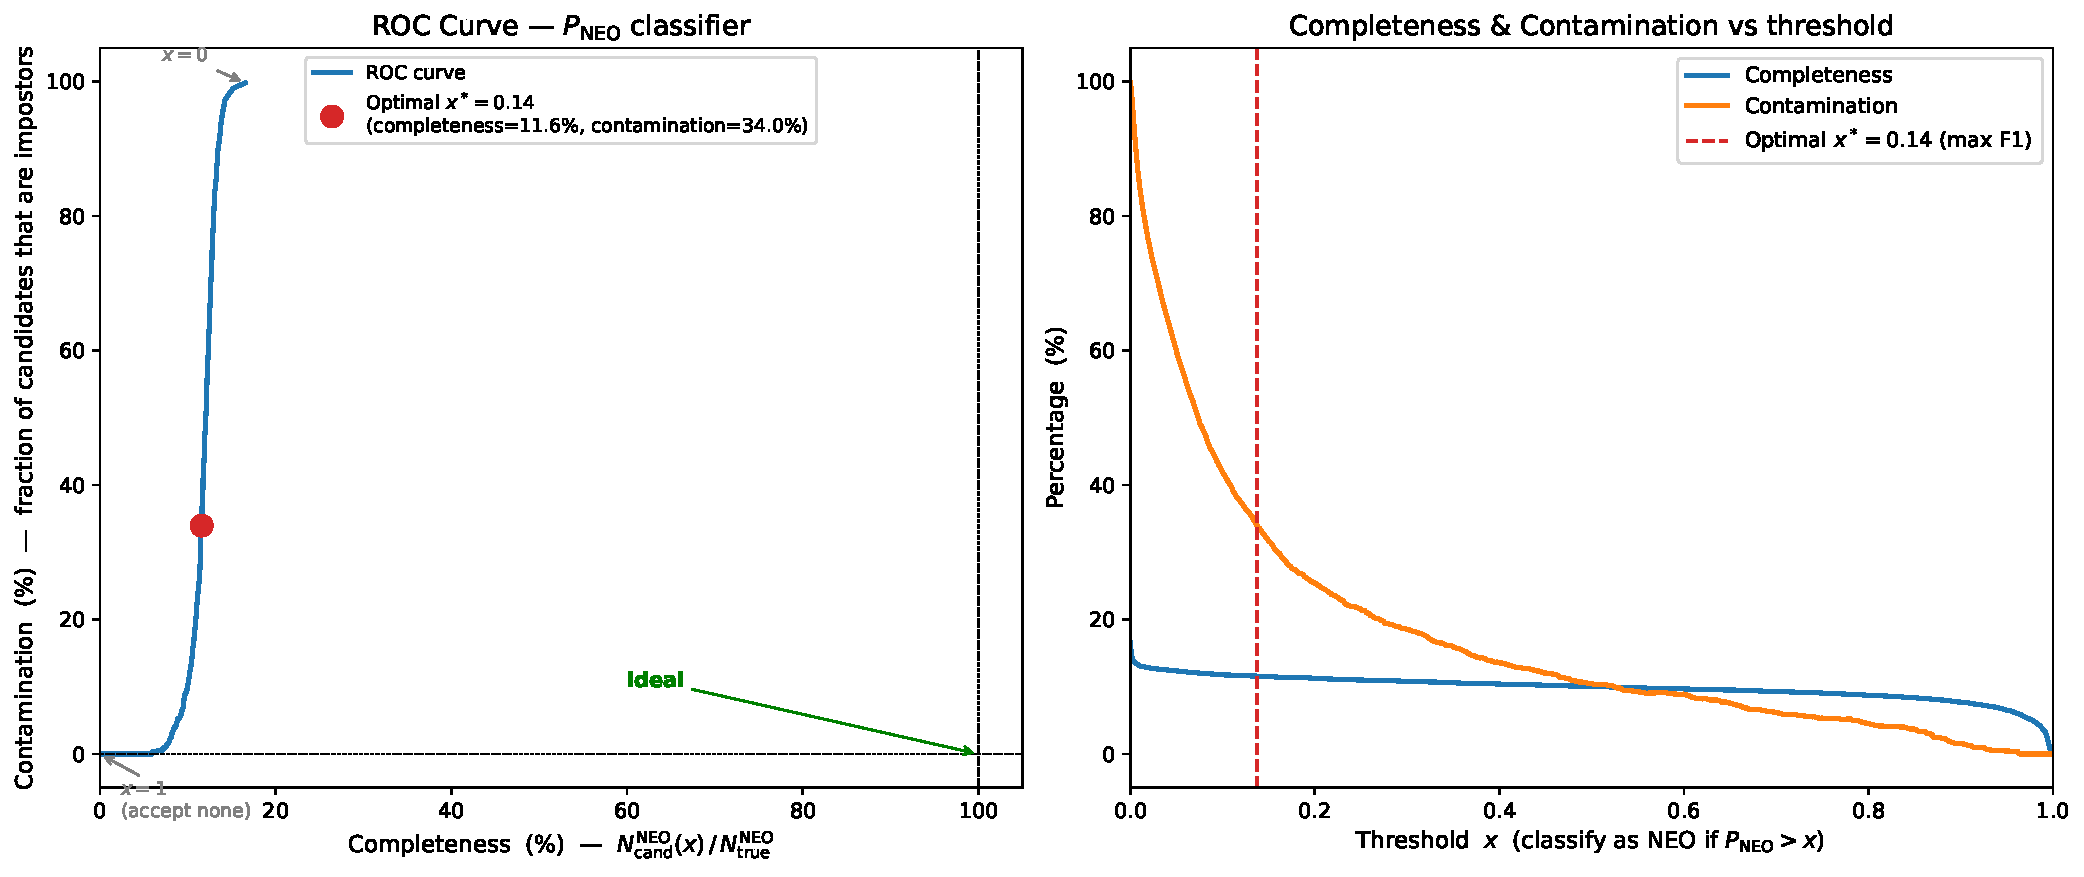
\includegraphics[width=\textwidth]{roc_curve.png}
\caption{
Receiver Operating Characteristic (ROC) analysis for the NEO classifier applied to the full four-population S3M sample visible in the anti-solar sky patch ($30^\circ$ radius, 2025 March 21).
\textit{Left:} ROC curve showing completeness (fraction of true NEOs recovered) versus contamination (fraction of candidates that are impostors) as the classification threshold $x$ is varied from 0 to 1.
The optimal threshold $x^* = 0.137$ (red point, maximising F1-score) achieves $11.6\%$ completeness and $34.0\%$ contamination (purity $= 66.0\%$).
\textit{Right:} Number of NEO candidates (true positives) and non-NEO candidates (false positives) as a function of $x$.
All false positives at the optimal threshold are MBAs; the NEO sky-plane velocity distribution overlaps substantially with the MBA distribution, limiting the completeness achievable from sky-plane kinematics alone.
}
\label{fig:roc_curve}
\end{figure*}

We note that the raw S3M NEO orbits were used throughout rather than the debiased NEOMOD3 model, having confirmed that the two populations produce nearly identical rate-of-motion distributions in the relevant velocity regions.
A future comparison using NEOMOD3 orbital weights would provide a direct test of sensitivity to the assumed NEO model.


\section{Results and discussion}
\label{sec:results}

\subsection{Comparison to digest2}
\label{sec:compD2}


\nopagebreak




\section{Conclusions}
\label{sec:conclusions}



\begin{acknowledgments}

\end{acknowledgments}


\begin{contribution}



\end{contribution}


\facilities{Vera C. Rubin Observatory, Minor Planet Center, JPL Small-Body Database Query}



\bibliography{bibliography}{}
\bibliographystyle{aasjournalv7}

\end{document}

% End of file `NEOrocks.tex'.
